\begin{frame}{Logical state}
\centering
\begin{tikzpicture}
	\def\width{4cm}
	\def\height{2cm}

	\only<1->{
		\node[align=center] (s1) {
			\ding{172} empty \\
			\begin{tikzpicture}[scale=0.5]
				\def\hist{2}
				\def\priv{2.8}

				\draw[step=1cm, gray] (0, 0) grid (\hist + \priv, 1) ;

				\fill[blue, opacity=0.2] (0, 0) rectangle (\hist, 1) ;
				\draw[very thick] (\hist, 1) -- ++(0, - 1) node[yshift=2mm, label=below:{\tiny front = back}] {} ;
				\fill[red, opacity=0.2] (\hist, 0) rectangle ++(\priv, 1) ;
			\end{tikzpicture}
	   } ;

	   \node[align=center] (s2) [right=\width of s1] {
	   		\ding{173} non-empty \\
			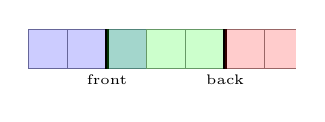
\begin{tikzpicture}[scale=0.5]
				\def\hist{2}
				\def\histx{1}
				\def\model{3}
				\def\priv{1.8}

				\draw[step=1cm, gray] (0, 0) grid (\hist + \model + \priv, 1) ;

				\fill[blue, opacity=0.2] (0, 0) rectangle (\hist + \histx, 1) ;
				\draw[very thick] (\hist, 1) -- ++(0, - 1) node[yshift=2mm, label=below:{\tiny front}] {} ;
				\fill[green, opacity=0.2] (\hist, 0) rectangle ++(\model, 1) ;
				\draw[very thick] (\hist + \model, 1) -- ++(0, - 1) node[yshift=2mm, label=below:{\tiny back}] {} ;
				\fill[red, opacity=0.2] (\hist + \model, 0) rectangle ++(\priv, 1) ;
			\end{tikzpicture}
	   } ;
   }

   \only<3->{
	   \node[align=center] (s3) [below=\height of s2] {
	   		\ding{174} emptyish \\
			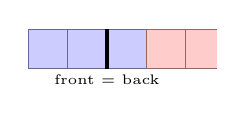
\begin{tikzpicture}[scale=0.5]
				\def\hist{2}
				\def\histx{1}
				\def\priv{2.8}

				\draw[step=1cm, gray] (0, 0) grid (\hist + \priv, 1) ;

				\fill[blue, opacity=0.2] (0, 0) rectangle (\hist + \histx, 1) ;
				\draw[very thick] (\hist, 1) -- ++(0, - 1) node[yshift=2mm, label=below:{\tiny front = back}] {} ;
				\fill[red, opacity=0.2] (\hist + \histx, 0) rectangle ++(\priv - \histx, 1) ;
			\end{tikzpicture}
	   } ;
	   \node[align=center] (s4) [below=\height of s1] {
	   	\ding{175} super empty \\
			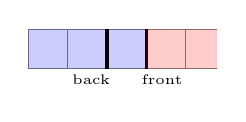
\begin{tikzpicture}[scale=0.5]
				\def\hist{2}
				\def\histx{1}
				\def\priv{2.8}

				\draw[step=1cm, gray] (0, 0) grid (\hist + \priv, 1) ;

				\fill[blue, opacity=0.2] (0, 0) rectangle (\hist + \histx, 1) ;
				\draw[very thick] (\hist, 1) -- ++(0, - 1) node[xshift=-2mm, yshift=2mm, label=below:{\tiny back}] {} ;
				\draw[very thick] (\hist + \histx, 1) -- ++(0, - 1) node[xshift=2mm, yshift=2mm, label=below:{\tiny front}] {} ;
				\fill[red, opacity=0.2] (\hist + \histx, 0) rectangle ++(\priv - \histx, 1) ;
			\end{tikzpicture}
	   } ;
   }

   \only<2->{
	   \draw[thick, ->] (s1) to[bend left] node[above] {\texttt{push}} (s2) ;
	   \draw[thick, ->] (s2) to[bend left] node[below] {\texttt{steal}} (s1) ;
	   \draw[thick, ->] (s2) to[looseness=3, out=135, in=45] node[above] {\texttt{push}, \texttt{pop}, \texttt{steal}} (s2) ;
   }
   \only<4->{
	   \draw[thick, ->] (s2) to[bend left] node[right] {\texttt{pop}} (s3) ;
	   \draw[thick, dotted, ->] (s3) to[bend left] node[below] {\texttt{pop}, \texttt{steal}} (s4) ;
	   \draw[thick, dotted, ->] (s4) to[bend left] node[left] {\texttt{pop}} (s1) ;
   }
   \only<5->{
   		\draw[thick, ->] (s1) to[bend left] node[right] {\texttt{pop}} (s4) ;
   		\draw[thick, dotted, ->] ([xshift=2mm]s1.south) to[bend left] ([xshift=2mm]s4.north) ;
   }

   \only<2-3>{
	   \matrix [below right, nodes={font=\tiny}] at (current bounding box.south west) {
	   		\draw[thick, ->] (0, 0) -- (1em, 0) node[right] {linearization} ; \\
	   } ;
   }
   \only<4->{
	   \matrix [right, nodes={font=\tiny}] at (current bounding box.south west) {
	   		\draw[thick, ->] (0, 0) -- (1em, 0) node[right] {linearization} ; \\
	   		\draw[thick, dotted, ->] (0, 0) -- (1em, 0) node[right] {stabilization} ; \\
	   } ;
   }
\end{tikzpicture}
\end{frame}
